\graphicspath{{Chapter1/Figs/}}

\chapter{Introduction}
\label{chapter1}
      	
   \vspace*{\fill}\par
   \pagebreak

\section{The Sun}

    \begin{figure}
        \centering
        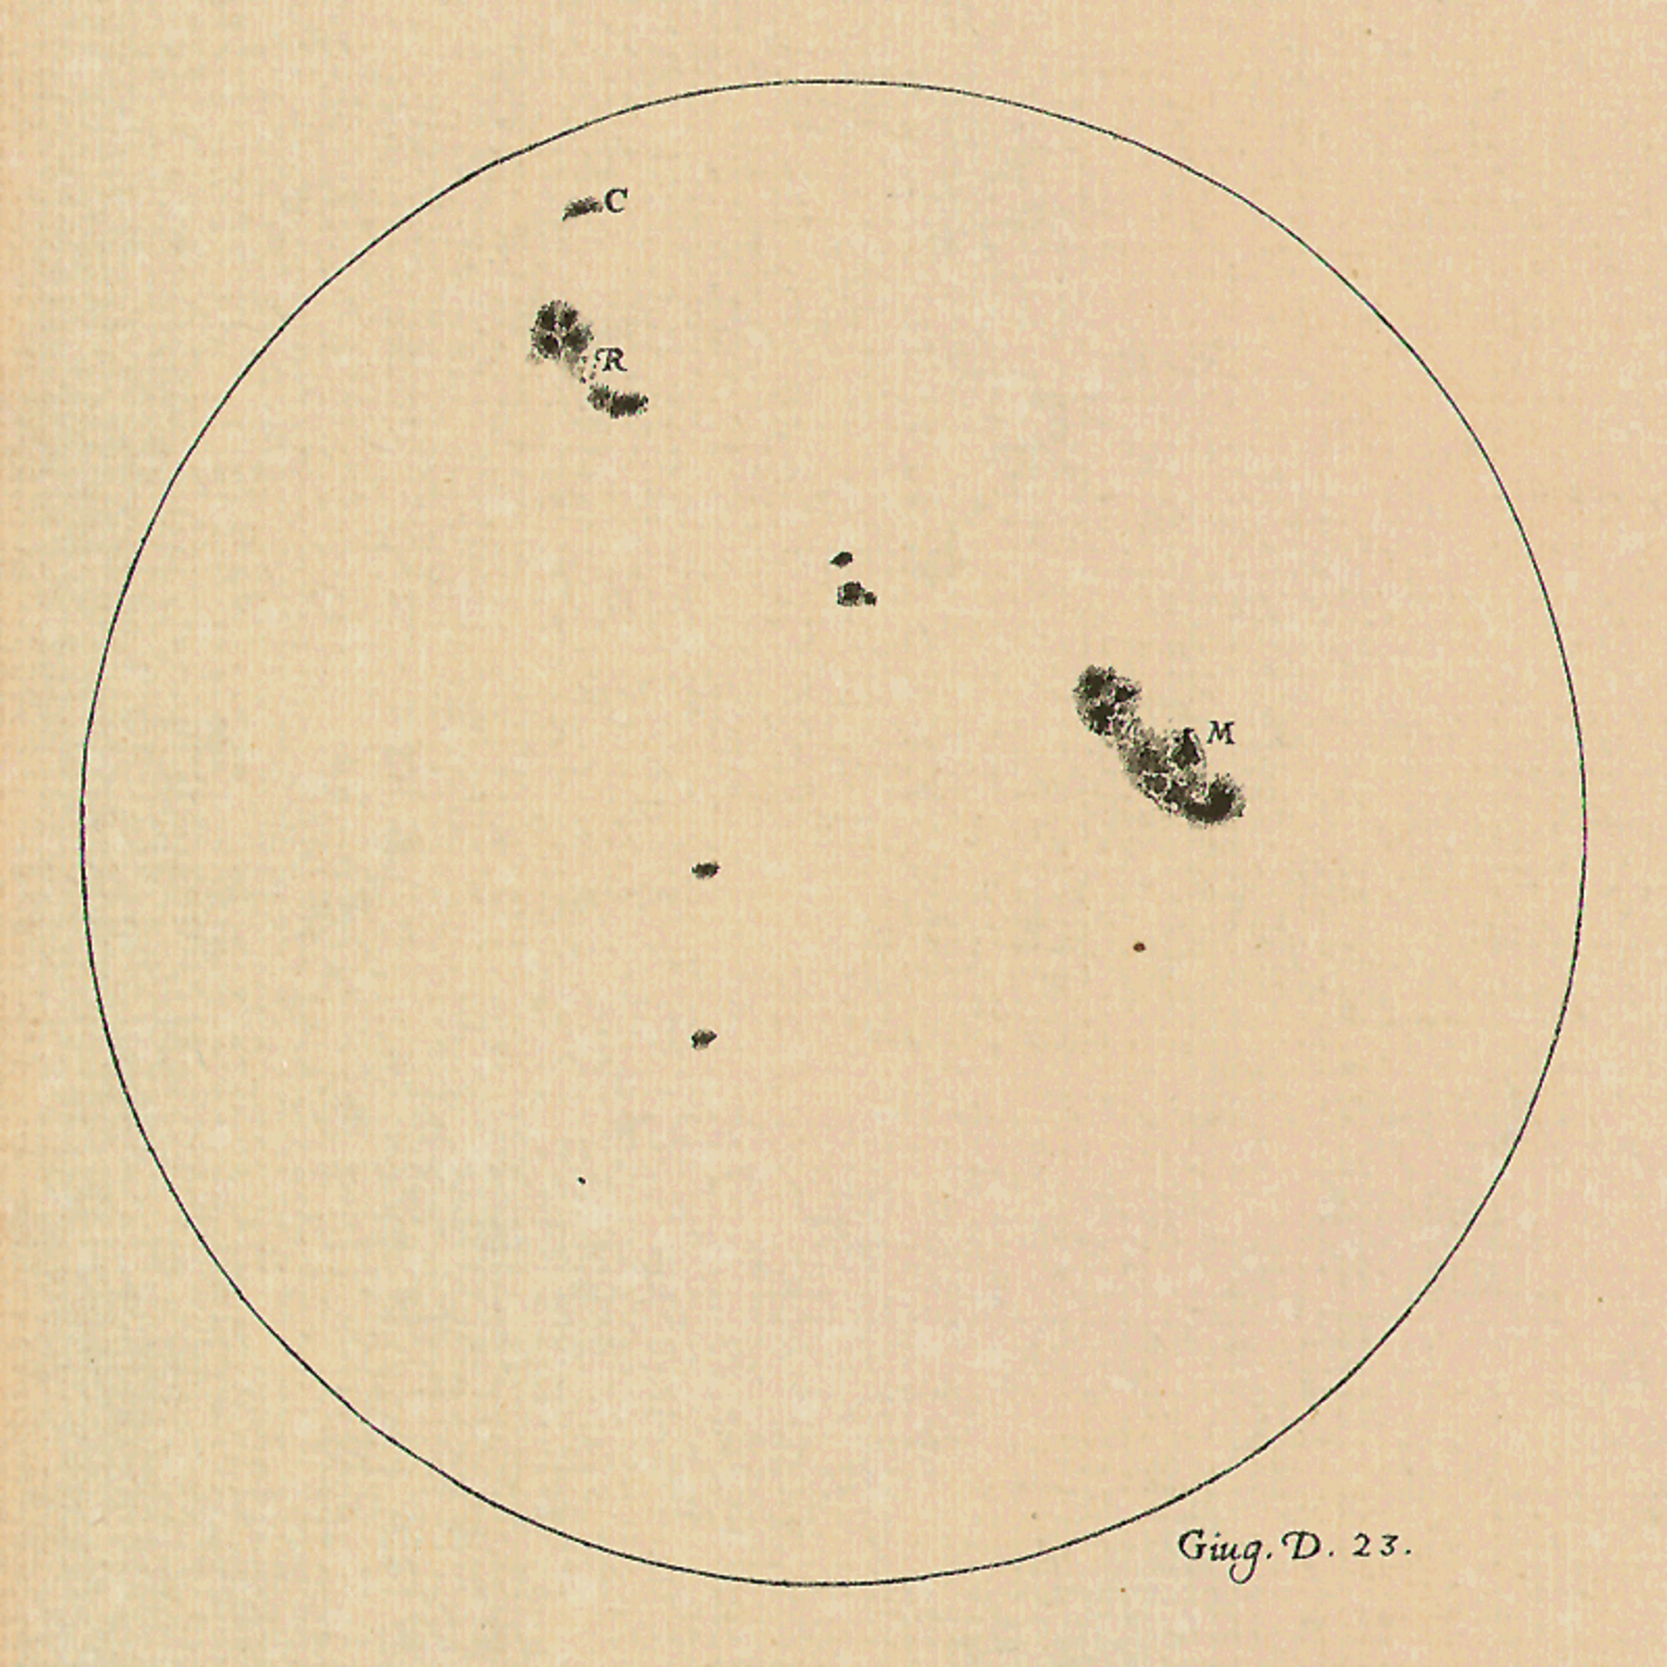
\includegraphics[width=\textwidth]{23_June_1613.pdf}
        \caption{
                A drawing of the solar surface by Galileo in the 17$^{\mathrm{th}}$ century. 
                The creation of the telescope forever changed astronomy.
                Here, the sunspot structure can be resolved; the inner (umbra) and outer (penumbra) regions can be seen clearly.
                Image credit goes to \cite{galileo}.
               }
        \label{fig:galileo}
    \end{figure}
     
    Our local star is known as the Sun and is a semi-common and uninteresting main sequence star (if you happen to be an astrophysicist).
    However to the general public and more importantly solar physicists, it forms the backbone of their lives.
    From simply as mundane as waking up at sunrise to making a long and (hopefully) successful career out of studying the Sun.
    
    For early humans, it appeared as a giant ball in the sky that seemed to revolve around the Earth and it defied any human understanding.
    Since the dawn of mankind, the mythology surrounding the Sun has been numerous.    
    From the New World, the Aztec's had a Sun god called Tonatiuh. 
    Without constant human sacrifice (mainly their enemies), they believed that the Sun would not move through the sky.
    From the Far East, the Chinese originally had 10 suns who took turns moving through the sky. 
    However, these suns were mischievous and decided to all appear at the same time. 
    This made life utterly unbearable on Earth, so an archer bestowed with a unique bow shot down 9 of the suns, leaving the one Sun we have today.
    From the Old World, the Greeks and Romans believed in Apollo who is the son of Zeus and Leto.
    He was known as the god of music, healing, light, truth and the Sun; a very busy god.
    With the decline of polytheism and the rise of monotheism, these gods and stories quickly became consigned to history. 
    For a review of many more solar mythologies, see \citet{mythbook}.
    
    The Sun had always been observed with the naked eye, sunspots had been visible and recorded by the ancient Chinese, further, many solar calenders were created to order human society.
    However, no systematic studies of the Sun had ever taken place.
    It took the enlightenment in Europe to mark the start of a transformation of society which led to the invention of the telescope (among other things).
    This is what started modern astronomy.
    
    The telescope was the device that allowed humanity's knowledge of our solar system to radically change.
    It was possible to observe the Sun in much greater detail for the first time.
    Galileo drew many full disc images of the Sun and Figure \ref{fig:galileo} is one such example. 
    With the telescope, the umbra and penumbra of sunspots was easily differentiated for the first time.
    Further, magnetic pores can be seen in the image.
    From here, many other discoveries were made such as the sunspot cycle, differential rotation and solar flares.
    With more time and a solar eclipse, layers of the solar atmosphere were finally observed, such as the chromosphere and the corona.
    The age of solar physics had finally begun.
    
    The scientific understanding of the Sun has advanced by leaps and bounds, especially during the past sixty years.
    This is mainly due to the launch of space missions, whether it was SkyLab or the numerous satellites now pointed at the Sun.
    The removal of the Earth's atmosphere was a decisive step, allowing the observation of spectral lines not possible on Earth and vastly improving the quality of observational data.
    The solar physics community is hard at work analysing the massive amount of data that is available and expanding our knowledge of the Sun.   
    However, there are still crucial challenges to overcome.
    They have in essence become the holy grails of solar physics: how the corona is heated and what is the dynamo process behind the solar magnetic field.

\subsection{The structure of the solar interior}

    The Sun's internal structure is divided into four sections; the core, the radiative zone, the tachocline and finally the convective zone.
    While we cannot see these regions directly, the process of helioseismology, much like seismology on Earth, has allowed humanity to come to grips with these layers and processes that occur within the Sun.
    Figure \ref{fig:Sun} showcases the multi-layered structure of the Sun.
    The image starts from the core, through the various interior layers until it reaches the solar atmosphere and the interplanetary medium.
    This picture of the Sun has been built up over time as observations and the mathematical models of the Sun have improved. 
    
    \begin{figure}
        \centering
        \includegraphics[width=\textwidth]{sun.pdf}
        \caption{
                A schematic diagram of the interior and external layers of the Sun.
                Also shown are several features that occur within the solar atmosphere; sunspots, granulation, flares and prominences.
                Image credit to \cite{sun_image}.
               }
        \label{fig:Sun}
    \end{figure}

\subsubsection{The core}

    The core is the beating heart of the Sun, the largest fusion reactor this side of Centaurus.
    The core has more than 60\% of the total mass of the Sun and extends roughly to 25\% of the total radius of the Sun.
    It has a density of around 150000 kg m$^{-3}$ and a temperature around 16 MK \citep{0004-637X-699-2-1403}.
    The fusion reactions occurs due to the high pressure and temperatures that exist in the core, which are enough to force the hydrogen atoms together. 
    This process which accounts for the vast majority of the energy generated, creates a range of high energy particles such as photons and neutrinos.
    
\subsubsection{The radiative zone}

    Due to the intense heat and the large pressure within this region, thermal radiation is the only mechanism able to transfer the heat generated by the core.
    The process of radiative transfer within the radiative zone happens on very small scales.
    Photons are emitted and absorbed on very short time-scales. 
    This means that it takes hundreds of thousands years for photons to exit this layer, which extends to about 70\% of the solar radius \citep{cox1991solar}. 
        
\subsubsection{The tachocline}

    The tachocline is the region that separates the radiative zone and the convective zone.
    It is very thin, being only 0.04\% of the solar radius.
    It has been long hypothesised that the solar magnetic field is created within this layer via a dynamo process \citep{soward2005fluid}.

\subsubsection{The convection zone}

    From the tachocline, the temperature and pressure has decreased enough to allow the fully ionized molecules to retain some electrons and thus the opaqueness of the plasma increases.
    This traps part of the radiative energy from below setting up a temperature gradient sufficient enough to allow convection to take place.
    Thermal columns are created, which carry hot plasma to the surface of the Sun and once it cools, it sinks back to the base of the convection zone.
    This process is believed to cause gravity waves within the solar interior which have yet to be observed.
    The visible effect of convection is the solar granulation pattern that can be seen in white light images of the Sun.  
    The pattern consists of cells that have a rough hexagonal shape. 
    At the top of the convection zone, the temperature drops to 5700 K and the density to 0.0002 kg m$^{-3}$ \citep{gai2000sun}. 
    A very important factor about the convection zone is the matter of differential rotation.
    The Sun rotates not as a solid body as the Earth does but as a fluid as the Gas Giants do. 
    The rotation rate decreases from the equator where it is 25 days to around 34 days at the poles.
    
\subsection{The solar atmosphere}
 
    The solar atmosphere is quite unlike the Earth's.
    While they both have multiple layers, the characteristics are wildly different (as you would expect). 
    The top of the convection zone is the start of the first layer of the solar atmosphere.
    Here, the optical depth, the fraction of photons that can pass through the layer is $\lessapprox$1, roughly equating to a third of all photons will pass into space.
    This layer is called the photosphere.
    There are three more layers, the chromosphere, the transition region and the corona (see Figure \ref{fig:Sun}).
    Then the solar atmosphere transitions into the solar wind which fills the interplanetary medium.
    
\subsubsection{The photosphere}

    The photosphere comes from the ancient Greek word ``photos'' meaning ``light''.
    It is the visible surface of the Sun, that can be seen with the naked eye.
    The photosphere has an approximate thickness of 500 km with a starting temperature of 5700 K which drops as you move away from the surface, getting to approximately 4500 K.
    This part is called the temperature minimum and is generally taken to be the top of the photosphere.

    The structure of the photosphere is composed of convection cells called granules, which are on average 1 Mm in diameter.
    Observed flows within these cells show uprising hot plasma in the centre which pushes the cooler plasma to the edges of the cell before flowing downwards. 
    These granules are short-lived, with a lifetime less than 10 minutes, resulting in a repeating pattern at small-scales.
    These can be seen in the top image of Fig \ref{fig:photosphere}, within circle A.
    On larger scales, super-granule structures have been observed with a 30 Mm diameter which can last for a day or longer \citep{lrsp-2010-2}.
    
    The convective nature of the Sun has allowed us to infer the interior structure. 
    The reason for this is that turbulence within the convection zone creates an entire spectrum of acoustic waves, named \textit{p}-modes, where \textit{p} stands for pressure.
    \textit{p}-modes penetrate into the solar interior and at certain frequencies, the waves become standing.
    This sets up many standing modes that can be measured on the photosphere, using line-of-sight Doppler images. 
    The mathematics used as a basis for this research is called spherical harmonics, and has allowed understanding of the many modes that are observed.
    The mode's overall properties are affected by the physical conditions where the maximum amplitude for that mode occurs. 
    This allows a building up of the information at each depth of the solar interior.
    
    The dynamics of the photosphere is governed by two processes; convection as discussed above, but also by the solar magnetic field.
    This makes understanding how the magnetic field is structured within the photosphere important. 
    The most common method employed in solar physics in order to measure the magnetic field is to exploit the Zeeman effect.
    This is the fact that when atoms are subjected to a magnetic field, their spectral lines split as a function of field strength and polarization.
    Unfortunately, this effect is only strong enough to be used in the photosphere where the magnetic field is strongest.
    However, many solar physicists have attempted measurements in various weak field areas \citep{1995ApJ...439..474M,1538-4357-613-2-L177,2008A&A...489L..57K}.
    These images are called solar magnetograms and they have revealed the basic magnetic field structure at the photosphere.
    The magnetic field is very weak ($\le 300$ Gauss) on average and is very sparse.
    This is referred to as the quiet Sun and is shown in the top image of Figure \ref{fig:photosphere}. 
    The structuring from convection can be seen clearly as well as several features (which are discussed below).
    As can be seen, the magnetic field does not clearly dominate as strongly as it does in other regions.

    \begin{figure}    
        \centering
        \begin{subfigure}[b]{0.75\textwidth}
            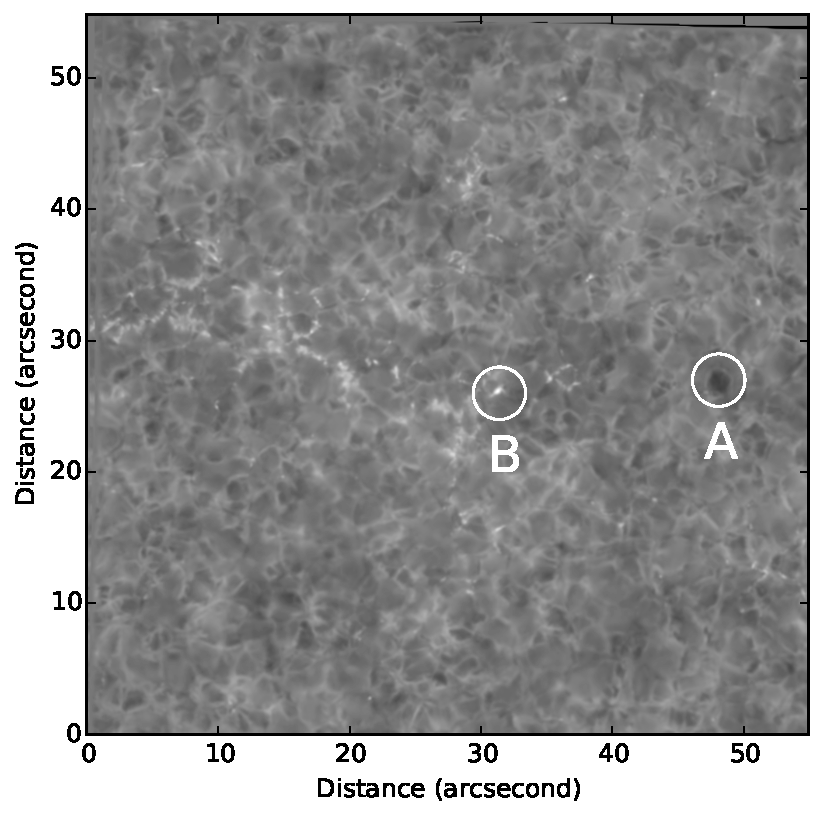
\includegraphics[width=\textwidth]{QS.pdf}
        \end{subfigure}\\~\\
        \begin{subfigure}[b]{0.75\textwidth}
            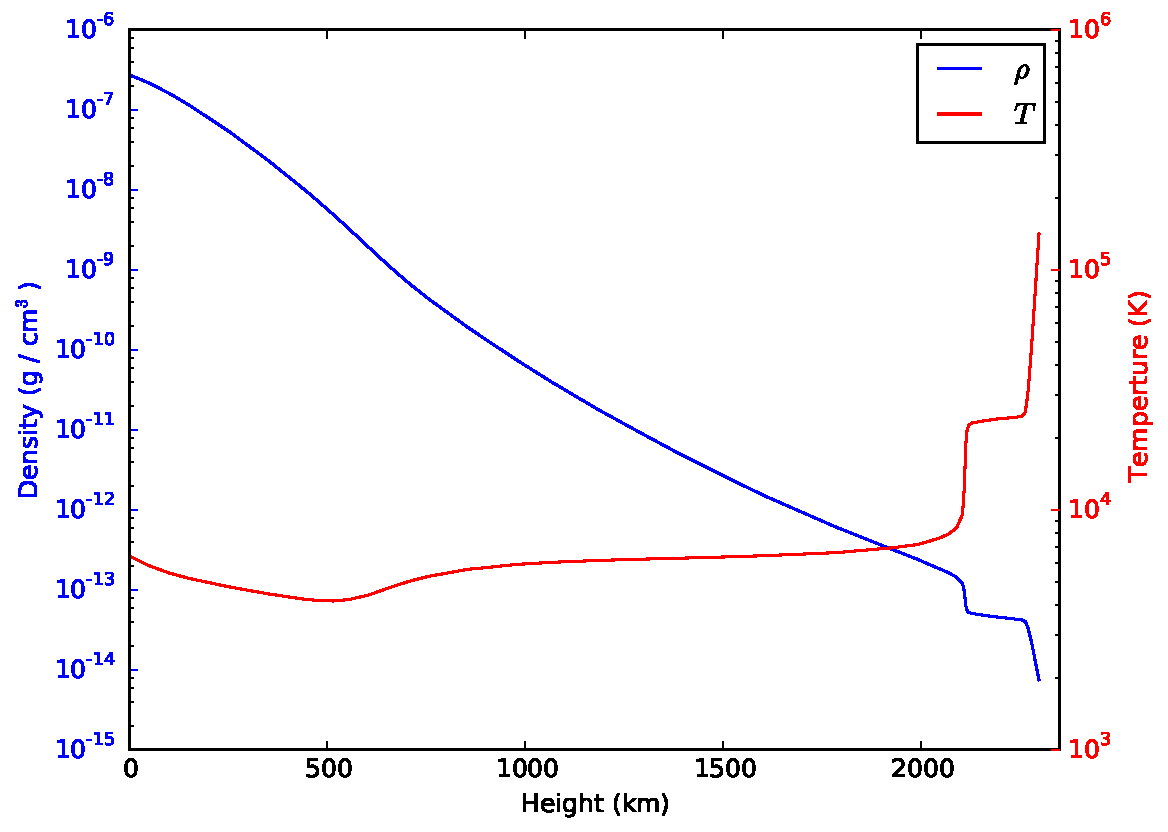
\includegraphics[width=\textwidth]{val3.pdf}
        \end{subfigure}
        \caption{
                \textit{(top)} Iron I ($630.2$ nm) image taken with the Swedish Solar Telescope on the $22^{\mathrm{nd}}$ of July 2012.
                It shows some of the features that are present in the quiet Sun: a granule cell (A) and a magnetic bright point (B).
                \textit{(bottom)} The VALIIIc \citep{1981ApJS...45..635V} model of the quiet Sun, density is in blue and temperature is in red.
                The temperature minimum region and the transition region can be seen clearly with these two parameters.
                }
        \label{fig:photosphere}        
    \end{figure}   
    
    Within the photosphere are small regions of concentrated magnetic field, named Magnetic Bright Points (MBPs).
    They are small-scale bright dots, as can be seen in Figure \ref{fig:photosphere}, in the circle labelled B.
    They are formed in the gaps between granule cells; the plasma flow has dragged the magnetic flux and thus becomes highly concentrated (>$1$ kG).
    The most likely reason for the increased brightness is that the flux tube has been evacuated of any plasma.
    As such, observations of MBPs allow a glimpse into the top of the convection zone, which has a higher temperature than the photosphere and is brighter.
    One important factor about MBPs was the observation of Alfv\'en waves \citep{Jess2009,Taroyan2009}.
    This was able to supply enough energy to the corona to overcome the ``Coronal Heating problem'' (detailed in section \ref{corona}).
        
    Active Regions (ARs) are areas of intense magnetic field concentrations on the Sun's surface.
    They are catalogued by the National Oceanic and Atmospheric Administration (NOAA) and are given numbers so they can be easily identified.
    ARs will vary in scale and what magnetic structures are present.
    Two of the most prevalent features within ARs are sunspots and magnetic pores.
    There are also many quiet Sun features and a whole raft of magnetic reconnection features. 
    The top image of Figure \ref{fig:AR_Num} displays one such AR. 
    It consists of $3$ sunspots, taken as the AR is about to disappear off-limb.
    Circle A encloses one of the sunspots, but by being able to use a different wavelength filter we can observe an Ellerman Bomb (B) and a jet event (C).
    The last two events are associated with magnetic reconnection \citep{2013SoPh..283..307N,2013A&A...560A..31N,2013ApJ...779..125N,2015ApJ...798...19N}.
     
    \begin{figure}
        \centering
        \begin{subfigure}[b]{0.75\textwidth}
           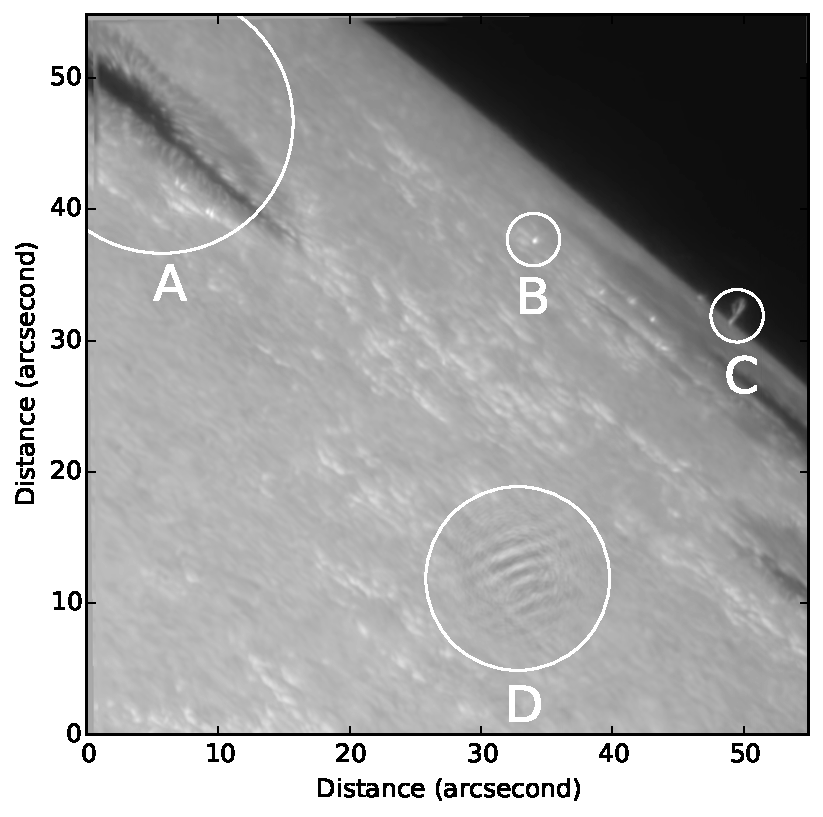
\includegraphics[width=\textwidth]{AR.pdf}
        \end{subfigure}\\~\\
        \begin{subfigure}[b]{0.75\textwidth}
           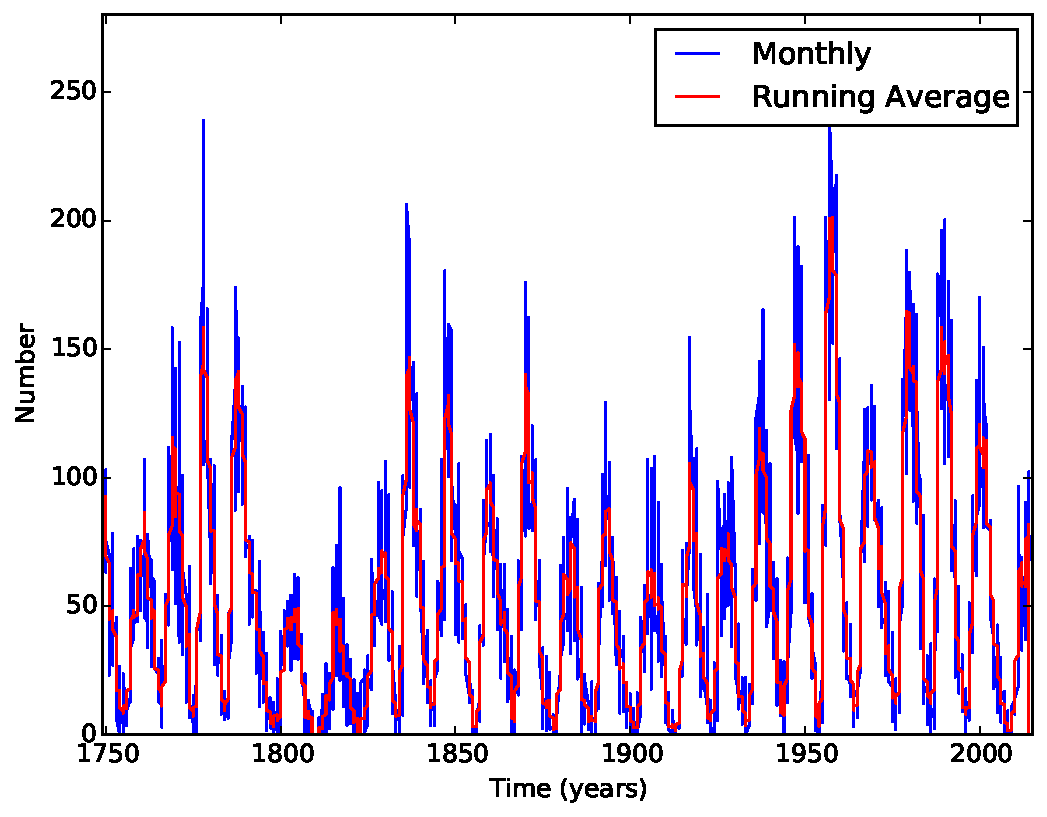
\includegraphics[width=\textwidth]{sunspot_number.pdf}
        \end{subfigure}
        \caption{
               \textit{(top)} An image of an active region (NOAA 11504) sunspot taken at the Swedish Solar Telescope using the Crisp Imaging SpectroPolarimeter on the $21^{\mathrm{st}}$ June. 
               The filter used is H$\alpha$ but into the far wings such that strong photospheric features can be observed.
               It shows some of the features that are present in Active Regions; sunspot (A), Ellerman Bomb (B), a jet (C) and seeing effects (D).            
               \textit{(bottom)} The sunspot number record as it currently stands since continuous tracking.  
               The eleven year solar cycle is clearly visible.
              }
        \label{fig:AR_Num}
     \end{figure}    
    
    When using a wavelength filter that resolves higher temperature plasma ($\ge1$ MK), loop structures can be see that rise several mega-meters in height.
    These are called coronal loops and they display a wide range of oscillations.
    Seismology of these loops, has estimated the background quantities such as density and magnetic field strength of these loops (see \cite{2005RSPTA.363.2743D} or \cite{Banerjee2007} for a detailed review). 
    These regions will also be the areas where flares or coronal mass ejections will originate from, since they contain large amounts of stored magnetic energy.

    These are the most spectacular events produced by the Sun.
    The amount of mass and energetic particles ejected can be considered scary. 
    These events have a direct impact on the Earth if the ejected material reaches Earth, f rom simply creating the aurora near the poles or in certain situations the disruption of radio transmissions, damage to satellites and electrical transmission lines.
    So it is important to understand the formation mechanism of these events so we can predict them and take measures to limit their damage.
    This is partly the realm of space weather research. 
    
    Sunspots are the strongest magnetic field concentrations on the solar surface.
    They have field strengths up to $4$ kG, they can span up to $20$ Mm in diameter.
    With the naked eye, they may appear to be dark spots, but with a good telescope, the sunspot structure can be seen to be divided into two parts.
    The first is the umbra which is the core of the sunspot, it is the coolest region ($\approx 4000$ K), as it is where the magnetic field is strongest and vertically inclined.
    The reason for the temperature difference between the sunspot and photosphere is that the magnetic field inhibits convection.
    This allows the plasma to cool down as no new hot material is being supplied.
    The second region is the penumbra and is made of elongated structures.
    Here the magnetic field is very inclined and weaker and fans around the umbra.

    Sunspot formation is a hotly debated topic (as much things are in solar physics).
    One current hypothesis about their formation is as follows.
    The magnetic field of the Sun is strongly polarised and with differential rotation, these magnetic fields lines become bunched together, increasing the local magnetic field strength.
    This effect creates a buoyancy force which slowly makes this newly created flux region rise towards the surface until it penetrates into the photosphere.
    It should be noted, however, that a complete understanding of how sunspots form has not yet been achieved and the mechanism is likely to be more complex than the one described above.
    In fairness of balance, other hypotheses are available.
    A more thorough review of the formation, evolution and unanswered questions relating to sunspots can be found in e.g. \cite{SAO}.
    
    The solar cycle is an $11$ year variation that the Sun undergoes where the polarity of the magnetic field flips.
    It is generally taken as $22$ years since that returns the magnetic field back to it's original polarity.
    The cycle does not have the same pattern or take the same amount of time each cycle.
    Generally, we have a solar maximum and a solar minimum.
    As the name suggests, we have a large amount of ARs and magnetic activity at a solar maximum, while this is reduced in a solar minimum.
    The solar cycle can be seen in the amount of sunspots which are visible (i.e., the amount of ARs that form).
    This has been counted since the 17$^{\mathrm{th}}$ century and it is called the sunspot number catalogue.
    The bottom image of Figure \ref{fig:AR_Num} displays this catalogue with the raw count as the blue line and a running average in red.
    This shows that the amount of sunspots varies with the cycle and that cycles can vary in length.
    Associated with the solar cycle is the variation in the number of ``extreme'' events, (flares and coronal mass ejections) and affects the overall structure of the solar atmosphere.
        
    Closer to home, it also changes the amount of solar radiance and solar UV/EUV that reaches the Earth.
    Sunspots are directly linked to the Earth's climate by the solar cycle \citep{FRIIS-CHRISTENSEN01111991}.
    This can directly impact the Earth's climate, as shown by the Maunder Minimum, which was an abnormally low amount of sunspots during the late seventeenth century and was the suspected cause of the ``Little Ice Age''.
   
    Sunspots have been under near constant observation.
    There are three main sunspot phenomena: 3 minute (5 mHz) and 5 minute (3 mHz) oscillations and running penumbral waves (RPWs).
    The first two are observed with a line-of-sight analysis, i.e, frequency filtering using the Fast Fourier Transform (FFT) (which is covered in Chapter 2).
    However, there is some evidence to suggest the existence of longer period oscillations \citep{LPO,SOS,Chorley2011}.
    The source of the 5-minute oscillations is thought to be a result of forcing by the 5-minute \textit{p}-mode global solar oscillation \citep{OWS,WAUO}.
    The 5-minute oscillations are typically seen in lines which form low in the cool umbral photosphere and are moderately suppressed not only in the penumbra, but also in the chromospheric atmosphere above the umbra \citep{OASO}.
    The cause of the 3-minute oscillations is still unknown but there are two main theories: they are either standing acoustic waves which are linked to the resonant modes of the sunspot, or, they are low-$\beta$ slow magneto-acoustic waves guided along the ambient magnetic field \citep{UTMO,OWS,OASO,ORWS}.
    The 3-minute oscillations are seen in elements that form higher up, in the low chromosphere, and these are also moderately suppressed in the penumbra \citep{OASO}.
    However, it should not be assumed that the period of these waves forms one finite peak in a power spectrum; generally, the immediate spectral area around these periods has several peaks clustered tightly together.
    A review of sunspot oscillations can be found in \citep{OASO} and a review of solar oscillations can be found in \citep{SO}.

    Magnetic pores can be considered as smaller scale sunspots without a penumbra, sometimes referred as ``naked umbra''.
    They share many general properties with sunspots, for example, they display similar line-of-sight oscillations.
    Due to their small size, magnetic pores have not been under as much observation as sunspots since it took a new generation of solar telescopes to resolve them clearly.
    One example of a magnetic pore can be seen in Figure \ref{fig:chromosphere}, which is studied in Chapter \ref{chapter5}.
    But this image is in the H$\alpha$ core which samples the chromosphere which is discussed below.
        
\subsubsection{The chromosphere}
\label{chromo}

    \begin{figure}
        \centering
        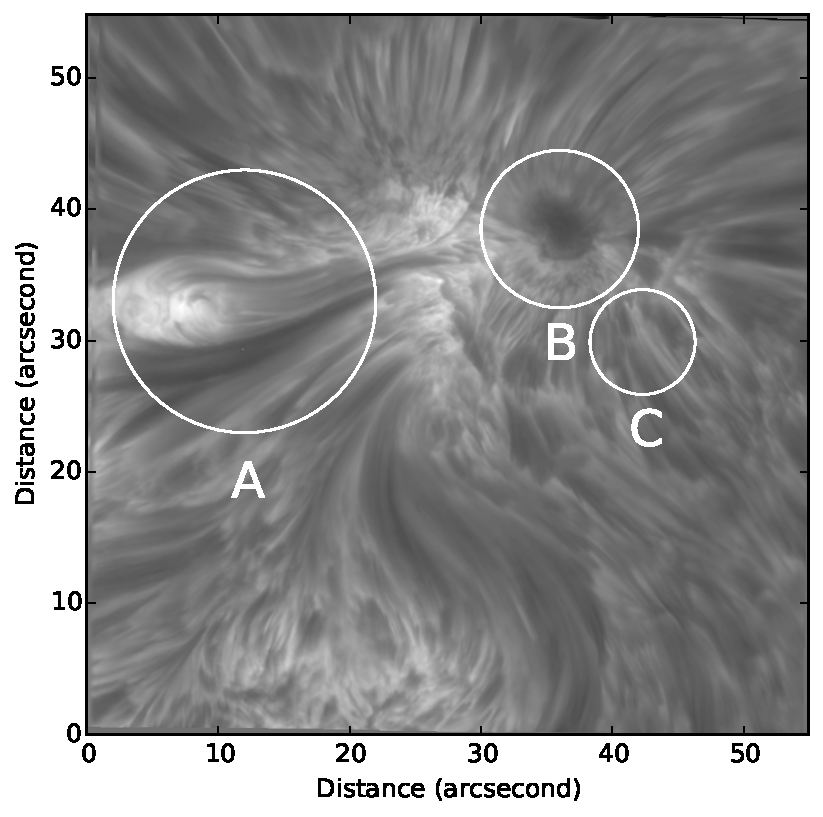
\includegraphics[width=\textwidth]{Chromo.pdf}
        \caption{
                 A H$\alpha$ line core image of Active Region NOAA 11510 observed on the 22$^{\mathrm{nd}}$ June 2012.
                 Here, this AR has a large pore that displays Running Penumbral waves (the focus of Chapter \ref{chapter5}).
                 Highlighted here are fibrils (A), the magnetic pore (B) and dynamic fibrils (C).
                 The complex nature of the chromosphere can be seen in detail and it still needs a full explanation.
                }
        \label{fig:chromosphere}
    \end{figure}   

    The next layer is visible from Earth during a total eclipse of the Sun as an intense red region giving it the name the chromosphere, from the Greek word ``chroma'', meaning colour.
    It is roughly $2$ Mm thick and is a highly complex layer.
    The temperature of the chromosphere increases with height and reaches around $20,000$ K at the boundary where it meets the next layer, the transition region.    
    The chromosphere has many small-scale structures that have been discovered over the past few decades.
    it is best observed in H$\alpha$ (a Hydrogen electron shell transition), where you can see these features but also another wavelength, Ca II K. 
        
    There are various names for these small-scale structures; spicules, fibrils, mottles and straws.
    The prevailing hypothesis is that there are two spicule types.
    Type I spicules are mainly seen in ARs but are scattered loosely elsewhere in the solar atmosphere.
    They can reach speeds up to $50$ km s$^{-1}$ and heights of $5$ Mm before falling back down, with typical lifetimes of $3$ to $10$ minutes, diameters of $120$ to $700$ km and temperatures of $10$ to $15$ kK.
    On disc, they are called dynamic fibrils and called mottles in the quiet Sun.
    Fibrils tend to be more elongated than mottles which are shorter.
    
    Type II spicules are located more often in the quiet Sun.
    They are faster (up to $150$ km s$^-1$), longer (up to $10$ Mm) and have a significantly reduced lifespan (up to $150$ s) when compared to Type I spicules.
    On disc, they are referred to as straws or more commonly Rapid Blue-shift Events (RBEs) \citep{Zaqarashvili2009}.
    Finally there is another fibril type that are long and mostly horizontal and longer-lived than dynamic fibrils.
    Some of these features are highlighted in Figure \ref{fig:chromosphere}.
    The circle A, has a good example of fibrils, long and fairly static, while circle C, shows dynamic fibrils which continually moved and swayed under our observation.
    
    These structures have been under heavy investigation as a potential source of energy transport in the solar chromosphere.
    \cite{Morton2012} using ground-based observations discovered incompressible transversal motions for fibrils which match the ones observed for limb spicules which were interpreted as Alfv\'en waves \citep{DePontieu2007}.
    Further, fast compressive MHD waves were also observed.
    The estimation of the energy these waves carry is quite large but explaining how they dissipate this energy is unknown at this time.
    A review of oscillations in spicules can be found by \cite{Zaqarashvili2009}. 
      
    Running Penumbral Waves (RPWs), are a phenomenon discovered by \cite{Zirin1972} and \cite{Giovanelli1972}. 
    Observed in H$\alpha$ in sunspot penumbrae, they are seen as a wave train of enhanced darkness that goes from the umbra to the penumbra.
    They tend to be concentric and cover a large azimuthal angle.
    On average, they have a speed of $15$ to $20$ km s$^{-1}$ before slowing to $5$ to $7$ km s$^{-1}$ at the end of the penumbra.
    They have a period typically of $200$ to $300$ seconds. 
    Common interpretation is that much like the $3$-minute oscillations, they are slow magneto-acoustic wave propagating upwards along the inclined magnetic field and the radially outwards movement is actually a visual pattern \citep{UTMO,ORWS,OASO}.
    This is expanded on in Chapter \ref{chapter5}.
    
    Finally, we discuss the existence of a Moreton wave \citep{1960AJ.....65U.494M}.
    These are seen also in H$\alpha$ wings as a dark and then a bright front.
    They are observed to travel away from flaring regions and are generally confined to a specific arc.
    They are more of a pulse than a wave and can travel up to $2000$ km s$^{-1}$.
            
\subsubsection{The transition region}

    Above the chromosphere, is a thin ($\approx100$ km) layer where the temperature rises rapidly from 20,000 K to 1,000,000 K.
    This is called the transition region.
    The rate of the increase is exponential and the density in this region decreases at a similar rate.
    In the bottom image of Figure \ref{fig:photosphere}, which displays the temperature and density of a semi-empirical model of the quiet Sun, this behaviour can be seen.
    This clearly means that the region is very non-uniform and \citep{tian2009solar} suggest that the height varies depending on what is below.
    It cannot be observed from the surface of Earth, but can be from space-borne instruments sensitive to ultraviolet and extreme ultraviolet light.
    
    Spicules, as discussed above, rise to large heights and it had been hypothesized that the TR would be a boundary.
    The spicule should hit the TR and create some form of a disturbance.
    These were discovered and called Transition Region Quakes (TRQs), found using the Extreme-Ultraviolet Imaging Spectrometer (EIS) instrument on-board the Japanese satellite Hinode.
    Coupled with MHD simulations, the disturbance was identified as a fast magneto-acoustic-gravity wave \citep{0004-637X-743-1-14}.
    These events further cement the link between the lower solar atmosphere and the higher regions.
    
\subsubsection{The corona}
\label{corona}

    The next layer is the outer atmosphere of the Sun called the corona.
    It is most easily seen during a total solar eclipse, but also observable using a coronagraph.
    The average temperature of the corona is about 1-2 MK, however, it reaches as high as 8-10 MK.
    The sheer scale of the corona is impressive.
    It is large in volume and it continuously expands into the solar system (i.e the solar wind) and stops far past the orbit of Pluto.
    The mechanism which accounts for the high temperature of the corona is still unknown, but two main ideas are in contention.
    Magnetic reconnection; the ability for the magnetic field to change its topology to release energy into the local environment, in order to heat the local plasma, or, MHD waves travelling up from the photosphere and dissipating their energy into the surrounding plasma.
    
    In all likelihood, a combination of these two main ideas will be the source behind coronal heating.
    This topic has been heavily researched for many decades and you can see reviews by e.g. \cite{erdelyi2004heating,Parnell2012}.
    The most recent development has shifted the question, from ``how do you heat the corona?'' to ``how do you heat the chromosphere?''\citep{Aschwanden2007}.
    For example, many sources of energy exist for wave heating \citep{Parnell2012}.
    
    The corona is host to many structures, X-ray bright points, plumes, prominences, streamers, coronal loops and coronal holes.
    Coronal holes are open magnetic structures which give rise to the fast solar wind, while coronal loops are one of the best examples of large scale magnetic structures within the solar atmosphere.
    They are typically up to one solar radius long and have a temperature of $2$ to $3$ MK.
    
    For a long time, it was hypothesised that MHD waves would not be able to go into the corona as the cut-off frequency would stop them.
    The launch of the Transition Region And Coronal Explorer (TRACE) space solar telescope changed this \citep{TRACE,TRACE1}.
    Numerous MHD oscillations where observed; damped transversal oscillations \citep{8007,2002A&A...394L..39G}, standing fast kink waves \citep{1999ApJ520880A,1999Sci...285..862N,1999SoPh..187..261S}, standing acoustic modes \citep{2003A&A...406.1105W}, fast sausage \citep{2001MNRAS.326..428W,2002MNRAS.336..747W,2003A&A...406..709K}, fast kink waves \citep{2005A&A...430L..65V}, propagating acoustic modes \citep{1997ApJ...491L.111O,2000A&A...355L..23D,2002A&A...393..649M} and torsional modes \citep{1998A&A...337..287E}. 
    This lead to a large focus on coronal seismology; estimating the background properties of coronal loops using observed properties of the waves.
    See a review on this topic by \cite{lrsp-2005-3}.
    Finally, EIT waves discovered using the Extreme Ultraviolet Imaging Telescope (EIT) instrument on the Solar and Heliospheric Observatory (SOHO) space satellite \citep{1998GeoRL..25.2465T}.
    These are large single-pulsed propagating fronts which appear to move unhindered throughout the corona after a large-scale event (such as a flare).
    They are believed to be associated with Moreton waves.
        
    Overall, this has been a brief overview of the history of the Sun, its interior and atmosphere. 
    For a more detailed introduction to the Sun, see \cite{priest1984solar} or \cite{2014masu.book.....P}.
    
\section{MHD theory}

    The mathematical underpinning used in solar physics is called magnetohydrodynamics (MHD).
    It adds the effects of a magnetic field to the governing equations of fluid mechanics. 
    More accurately, it is the melding of Maxwell's equations to the Navier-Stokes equations.
    This is credited to Hannes Alfv\'en, who won a Nobel Prize in Physics for this major contribution to science \citep{1942Natur.150..405A,erdelyi2007}.

\subsection{MHD equations}

    One of the most repetitive parts in any solar physics thesis is what is about to follow.
    There are several equations that form the core of MHD and are solved in many different magnetic configurations. 
    The ultimate aim is to understand how these configurations will evolve in time or how they react to external factors.
    Further, they are solved to find out what kind of waves these configurations can support as well as how they disturb the equilibrium. 
    The MHD equations include many physical effects, however, we have taken the ideal assumption; adiabatic, inviscid, radiation, no thermal conduction and no resistivity.
    This is ideal MHD and the resulting equations are,
    \begin{align}                                                         
        \dfrac{\partial \rho }{\partial t} + \nabla \cdot (\rho \boldsymbol{\mathrm{v}}) =       
        0,\tag{Mass Conservation}\\                                  
        \rho \dfrac{\mathrm{D}\boldsymbol{\mathrm{v}}}{\mathrm{D}t} =
        -\nabla p + \dfrac{1}{\mu}(\nabla \times \boldsymbol{\mathrm{B}}) \times \boldsymbol{\mathrm{B}} + \rho \boldsymbol{\mathrm{g}},\tag{Equation of Motion}\\
        \dfrac{\mathrm{D}}{\mathrm{D}t} \left(\dfrac{p}{\rho^\gamma} \right)  = 0,\tag{Energy Equation}\\       
        \dfrac{\partial \boldsymbol{\mathrm{B}}}{\partial t} = \nabla \times (\boldsymbol{\mathrm{v}} \times \boldsymbol{\mathrm{B}}),\tag{Induction Equation}               
    \end{align}
    subject to
    \begin{align}
        \nabla \cdot \boldsymbol{\mathrm{B}} = 0,\tag{Solenoid Equation}\\
        p = \mathrm{k_B} \dfrac{\rho}{\mathrm{m}} \mathrm{T},\tag{Ideal Gas Law}\\  
        \boldsymbol{\mathrm{E}} = - \boldsymbol{\mathrm{v}} \times \boldsymbol{\mathrm{B}},\tag{Ohm's Law}\\
        \boldsymbol{\mathrm{j}} = \nabla \times \boldsymbol{\mathrm{B}}/ \mu.\tag{Electric Current}                          
    \end{align}
    Here $\rho$ is the density, $\boldsymbol{\mathrm{v}}$ is the velocity, $\frac{\mathrm{D}}{\mathrm{D}t}$ is the convective derivative $\left(\frac{\partial}{\partial t} + (\boldsymbol{\mathrm{v}}\cdot\nabla)\right)$, $p$ is the pressure, $\gamma$ is the ratio of specific heats ($5/3$), $\boldsymbol{\mathrm{B}}$ is the magnetic field, $\mathrm{k_B}$ is Boltzmann's constant, $\mathrm{m}$ is the mass, $\mathrm{T}$ is the temperature, $\boldsymbol{\mathrm{E}}$ is the electric field, $\boldsymbol{\mathrm{j}}$ is the current density and $\mu$ is the vacuum permeability. 

    There are actually eight partial differential equations for eight variables.
    Both $\boldsymbol{\mathrm{v}}$ and $\boldsymbol{\mathrm{B}}$ have three components each and we have the density and temperature.
    From this, the typical recourse is to examine the case of small perturbations for the MHD quantities, i.e.,
    \begin{align*}                                                         
        \boldsymbol{\mathrm{B}} &= \boldsymbol{\mathrm{B}}_0 + \boldsymbol{\mathrm{B}}_1(\boldsymbol{r},t)\\               
        \boldsymbol{\mathrm{v}} &= \boldsymbol{0} + \boldsymbol{\mathrm{v}}_1(\boldsymbol{r},t)\\               
        p &= p_0 + {p_1}(\boldsymbol{r},t)\\               
        \rho &= \rho_0 + {\rho_1}(\boldsymbol{r},t).\\              
    \end{align*}
    Here, subscripts are used to separate out the background ($\mathrm{B}_0$) and perturbation ($\mathrm{B}_1$) quantities.
    There is assumed to be no background flow and that all perturbations are much smaller than the background value (e.g., $\mathrm{B}_0 \gg \mathrm{B}_1$).      
    This leads to the linearised ideal MHD equations,
    \begin{align}                                                         
    \dfrac{\partial \rho_1 }{\partial t} + (\boldsymbol{\mathrm{v}}_1 \cdot \nabla)\rho_0 + + \rho_0 (\nabla \cdot \boldsymbol{\mathrm{v}}_1) =       
    0,\tag{Mass Conservation}\\                                  
    \rho_0 \dfrac{\partial \boldsymbol{\mathrm{v}}_1}{\partial t} =
    -\nabla p_1 + \dfrac{1}{\mu}(\nabla \times \boldsymbol{\mathrm{B}}_1) \times \boldsymbol{\mathrm{B}}_0 + \rho_1 \boldsymbol{\mathrm{g}},\tag{Equation of Motion}\\
    \dfrac{\partial p_1}{\partial t} + (\boldsymbol{\mathrm{v}}_1 \cdot \nabla)p_0 - c_s^2 \left( \dfrac{\partial \rho_1}{\partial t} + (\boldsymbol{\mathrm{v}}_1 \cdot \nabla)\rho_0 \right) = 0,\tag{Energy Equation}\\       
    \dfrac{\partial \boldsymbol{\mathrm{B}}_1}{\partial t} = \nabla \times (\boldsymbol{\mathrm{v}}_1 \times \boldsymbol{\mathrm{B}}_0),\tag{Induction Equation}\\
    \nabla \cdot \boldsymbol{\mathrm{B}}_1 = 0, \tag{Solenoid Equation}               
    \end{align}
    where we can define the first characteristic speed in MHD; the sound speed, $c_s^2 = {\gamma p_0}/{\rho_0}$.
    There is another important characteristic speed and that is the Alfv\'{e}n speed, $c_A^2 = {\mathrm{B}_0^2}/{\sqrt{\rho_0}}$.
    These equations need to then be applied to an equilibrium and, since the focus is sunspots and magnetic pores, a cylindrical flux tube is the ideal choice.
    
\subsection{MHD waves in cylindrical flux tubes}

    To understand the observed oscillations in sunspots and pores, it is important to investigate the nature of oscillations within an idealised model of these structures.
    The most iconic investigation into this was undertaken by Edwin and Roberts in 1983 \citep{WPMC}.
    Their analysis is based on the non-slender flux tube, where the tube radius is greater or equal to the wavelength of the oscillations.
    Further it ignores the effects of gravity (i.e. the stratification of the atmosphere), which is important when the wavelength is comparable to the atmospheric scale height and in the photosphere this is the case \citep{LNLMHD}. 
    It is important to note that in thin flux tubes, there are two other characteristic wave speeds.
    One is a subsonic, sub-Alfv\'{e}nic speed, $c_T$ (defined later on), and the other is the ``mean'' Alfv\'{e}n speed, $c_k$.

    The model is as follows; a cylindrical magnetic flux tube of radius $a$ with its own density ($\rho_0$), pressure ($p_0$) and magnetic field ($\mathrm{B}_0\textbf{\^{z}}$) is embedded in a magnetic environment with a similar profile ($\mathrm{B}_e \textbf{\^{z}}$, $\rho_e$ and $p_e$ ).   
    The density and pressure are uniform throughout the medium.
    The top image of Figure \ref{fig:fluxtube} is a schematic drawing of this model. 
        
    \begin{figure}
        \centering
        \begin{subfigure}[b]{0.75\textwidth}
            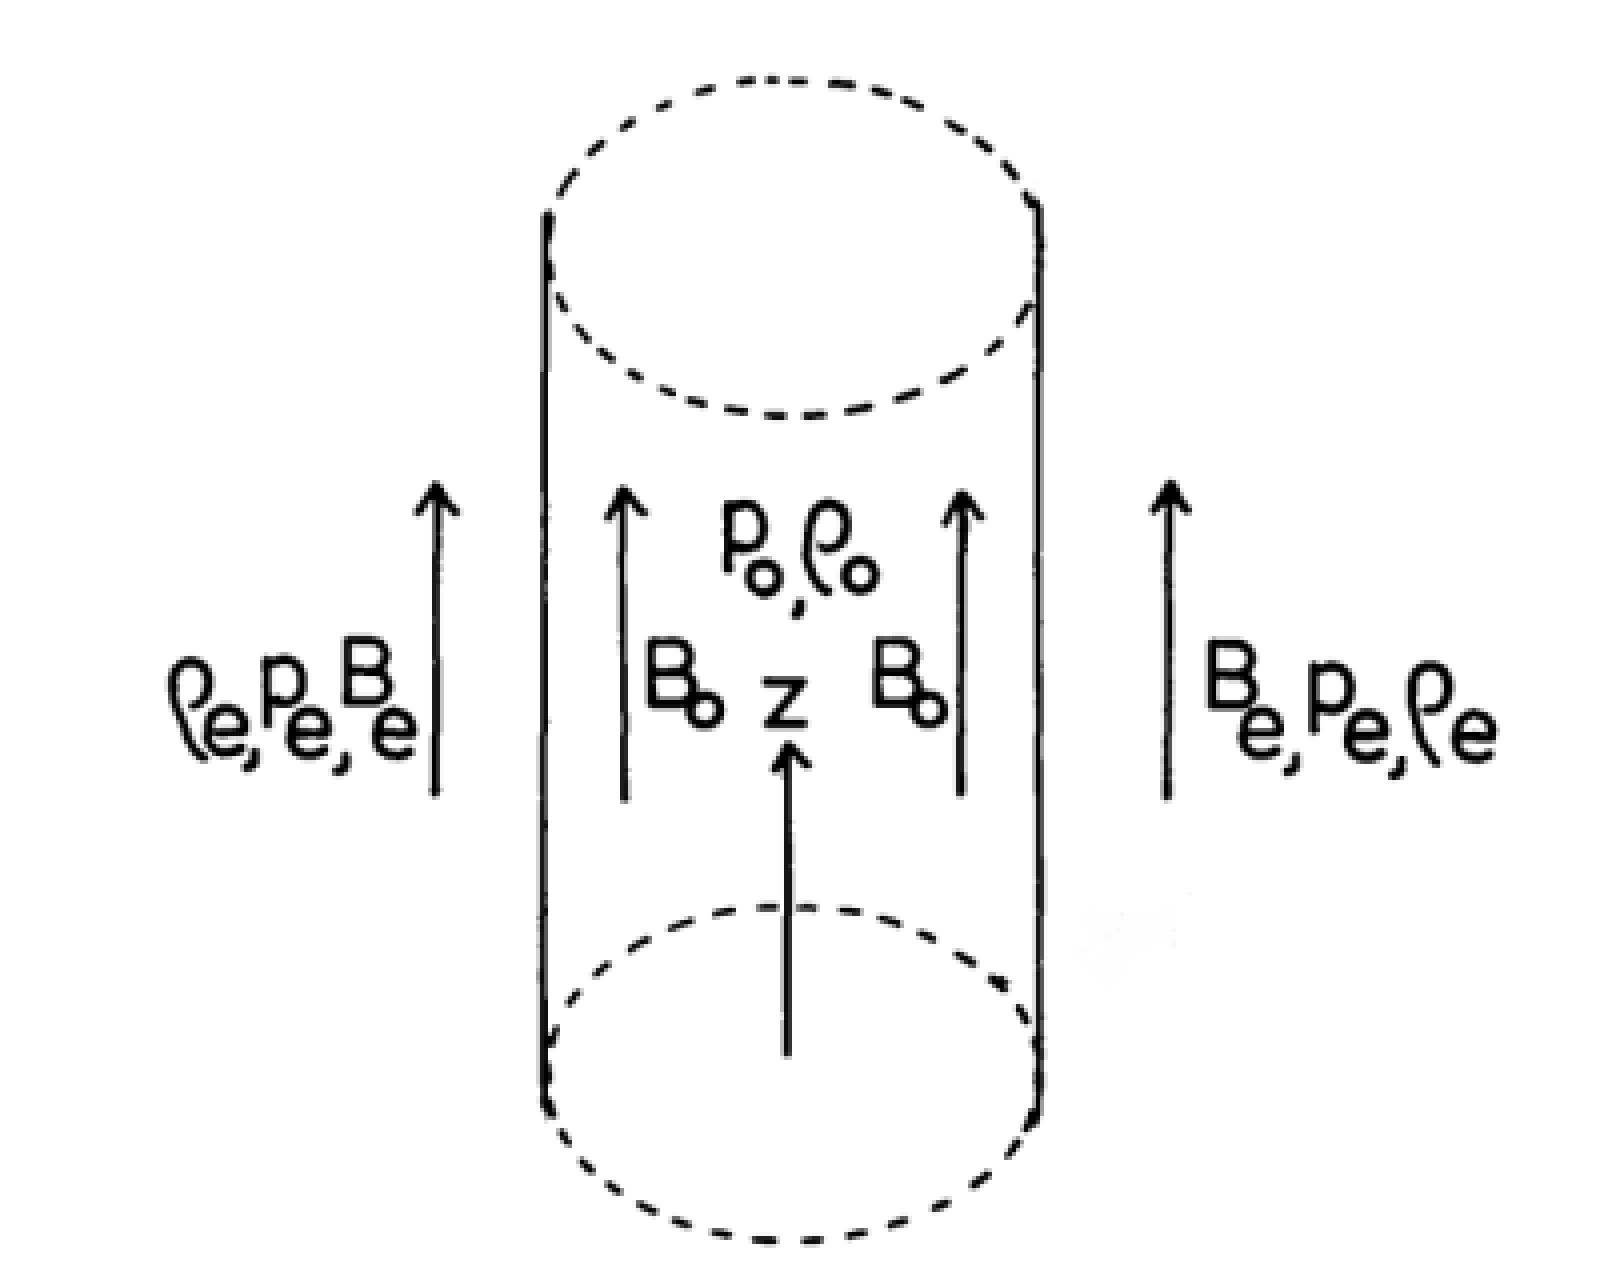
\includegraphics[width=\textwidth]{Fluxtube}
        \end{subfigure}\\~\\
        \begin{subfigure}[b]{0.65\textwidth}
            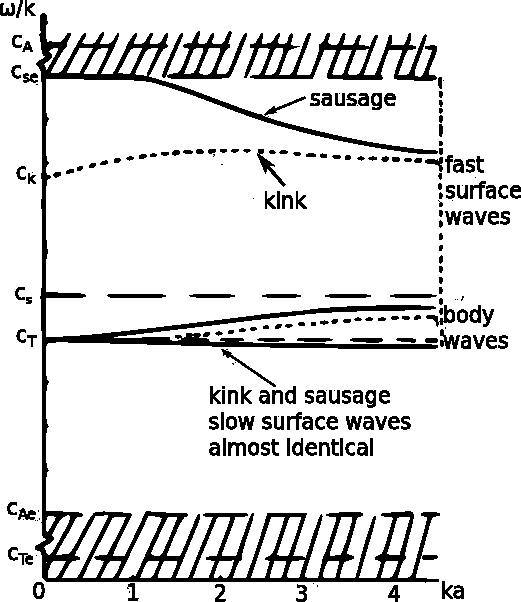
\includegraphics[width=\textwidth]{dispersion}
        \end{subfigure}
        \caption{
                \textit{(top)} The equilibrium conditions used to model wave behaviour in a magnetic flux tube.
                Image is a modified version of Figure 1 from \cite{WPMC}.
                \textit{(bottom)} The dispersion relationship derived from the MHD equations under photospheric conditions ($c_A > c_{se} > c_k > c_{Ae} $).
                The hatched areas are the excluded  values of $\omega$ and $ka$.
                Image is a modified version of Figure 2 from \cite{WPMC}.
                }
        \label{fig:fluxtube}
    \end{figure}
    
    This is the starting point for deriving the dispersion relation for MHD waves in a magnetic flux tube.
    It is assumed that this system is in equilibrium.
    Perturbations to the equilibrium conditions then add extra terms to the ideal MHD equations (i.e., the equations above).
    By introducing the Fourier decomposition of the perturbations, they show that the amplitude term is the Bessel equation.
    When bound on the axis of the cylinder ($r=0$), two solutions exist for either the body or surface wave.
    In the external atmosphere, the assumption of no propagation of energy away from or towards the cylinder allows the solution for the amplitude to be found for the external atmosphere.
    Further, the kinetic and magnetic energy density tend to zero as $r\rightarrow\infty$.
    Continuity at the boundary ($r=a$) has to be kept (radial velocity component $v_r$, and the total pressure) which yields the dispersion relations for surface waves and body waves \citep{WPMC}.
    These are,
    \begin{align}
        \rho_0 (k^2 c_A^2 - \omega)m_e \dfrac{K_n^\prime(m_e a)}{K_n(m_e a)} &= \rho_e (k^2 c_{Ae}^2 - \omega)m_0 \dfrac{I_n^\prime(m_0 a)}{I_n(m_0 a)} \tag{Surface, m$_0^2 > 0$} \\
        \rho_0 (k^2 c_A^2 - \omega)m_e \dfrac{K_n^\prime(m_e a)}{K_n(m_e a)} &= \rho_e (k^2 c_{Ae}^2 - \omega)n_0 \dfrac{I_n^\prime(n_0 a)}{I_n(n_0 a)} \tag{Body, m$_0^2 = -n_0 < 0$} 
    \end{align}
    where, $K_n$ and $I_n$ are Bessel functions of order n, $K_n^\prime$ and $I_n^\prime$ are the derivatives of the Bessel functions, $m_0$ and $m_e$ are the internal and external wavenumber, defined as, $$\dfrac{(k^2 c_{s}^2 - \omega^2)(k^2 c_{A}^2 - \omega^2)}{(c_{s}^2 + c_{A}^2)(k^2 c_{T}^2 - \omega^2)},$$ and $c_{T}$ is the tube speed, $$c_{T} = \dfrac{c_s^2 c_A^2}{c_s^2 + c_A^2}.$$
    Finally, these dispersion relations are solved under photospheric conditions and the solutions are plotted at the bottom of Figure \ref{fig:fluxtube}.
        
    These dispersion relations are important as they detail the way in which waves propagate through numerous flux tube sizes.
    It shows the limits of the wave solutions indicating in what regimes they cannot exist.
    Surface waves are dispersive as their phase speed depends on the wavenumber.
    There are slow body waves which are both sausage, kink and fluting modes; these modes have a phase speed between the tube and sound speeds.
    Slow surface waves have phase speeds close to the tube speed. 
    There is also a surface wave with a phase speed close to the kink speed and another surface wave near the sound speed.
    If one can measure the phase speed of an observed wave and the $ka$ of the flux tube, one can also likely identify the observed waves.
    
    One factor that has been neglected is the mode number ($n$), its value governs the way in which the wave disturbs the flux tube.
    This gives us the name; sausage ($n=0$), kink ($n=1$) and fluting ($n>1$).
    These different wave modes cause characteristic physical effects which can be used to identify each different wave mode.
    
    Figure \ref{fig:tube} shows the physical changes to the flux tube, caused by each different wave.
    The first diagram (a) shows how the slow wave affects the flux tube. 
    The velocity perturbation is longitudinal.
    When the flux tube contracts the density decreases indicating a phase difference of $\pi$, but also the same phase difference for the cross-sectional area and intensity.
    The second diagram (b) shows the fast sausage mode.
    Here the velocity perturbations are radial, as such when the flux tube contracts the density actually increases unlike the slow sausage mode.
    The cross-sectional area and intensity are in-phase, as well as the magnetic field.
    These diagrams have been improved over time and movies have been created which can be found within several papers \citep{Morton2012,jess2015multiwavelength} and online sources (\url{http://www2.warwick.ac.uk/fac/sci/physics/research/cfsa/research/wpc/vis/} or \url{http://swat.group.shef.ac.uk/fluxtube.html}).
    The main conclusion of \citet{Moreels2013b} is that fast and slow modes have a different phase behaviour, namely that slow modes have an in-phase behaviour (i.e. $0$ degrees phase difference between the area and the Lagrangian intensity oscillations), while fast modes have an anti-phase behaviour (i.e. $180$ degrees phase difference between the area and the Lagrangian intensity oscillations).
    Throughout most of this Thesis we use the Lagrangian intensity variations, i.e. the intensity variations when following the motion of the plasma. 
    Finally, the kink wave is non-compressible (to first order linear limit, long wavelength approximation) and perturbs the flux tube axis, as such, it is very difficult to measure directly unless it is possible to isolate the central axis of the flux tube, which is difficult for a sunspot or magnetic pore.
    This has been done for spicules and fibrils and as such, kink and Alfv\'en waves have been observed (see section \ref{chromo}).
  
    While these are toy arguments and descriptions, these phase relations have been derived by several authors \citep{PMHDW,Moreels2013,Moreels2013b,2015A&A...579A..73M}.
    They have taken complex models of embedded flux tubes to derive an almost full set of phase relations for many of the MHD wave modes and whether they are standing or propagating.  
    Table \ref{tab:phase} displays the phase relations between the intensity, Doppler velocity, magnetic field and for the cross-sectional area and intensity for each wave type and whether it is a standing or propagating wave.
    This table will be used later on in this Thesis in order to identify the observed oscillations which occur within the numerous magnetic structures analysed. 
    Since the focus has been on compressive perturbations, kink waves are neglected from this point onwards, as are Alfv\'en waves.
    However, see these recent review of both of these waves with regards to theory and observations \citep{Mathioudakis2013,jess2015multiwavelength}.
    It is important to note that the focus has been exclusively on MHD sausage waves within this Thesis.
    
    \begin{figure}
        \centering
        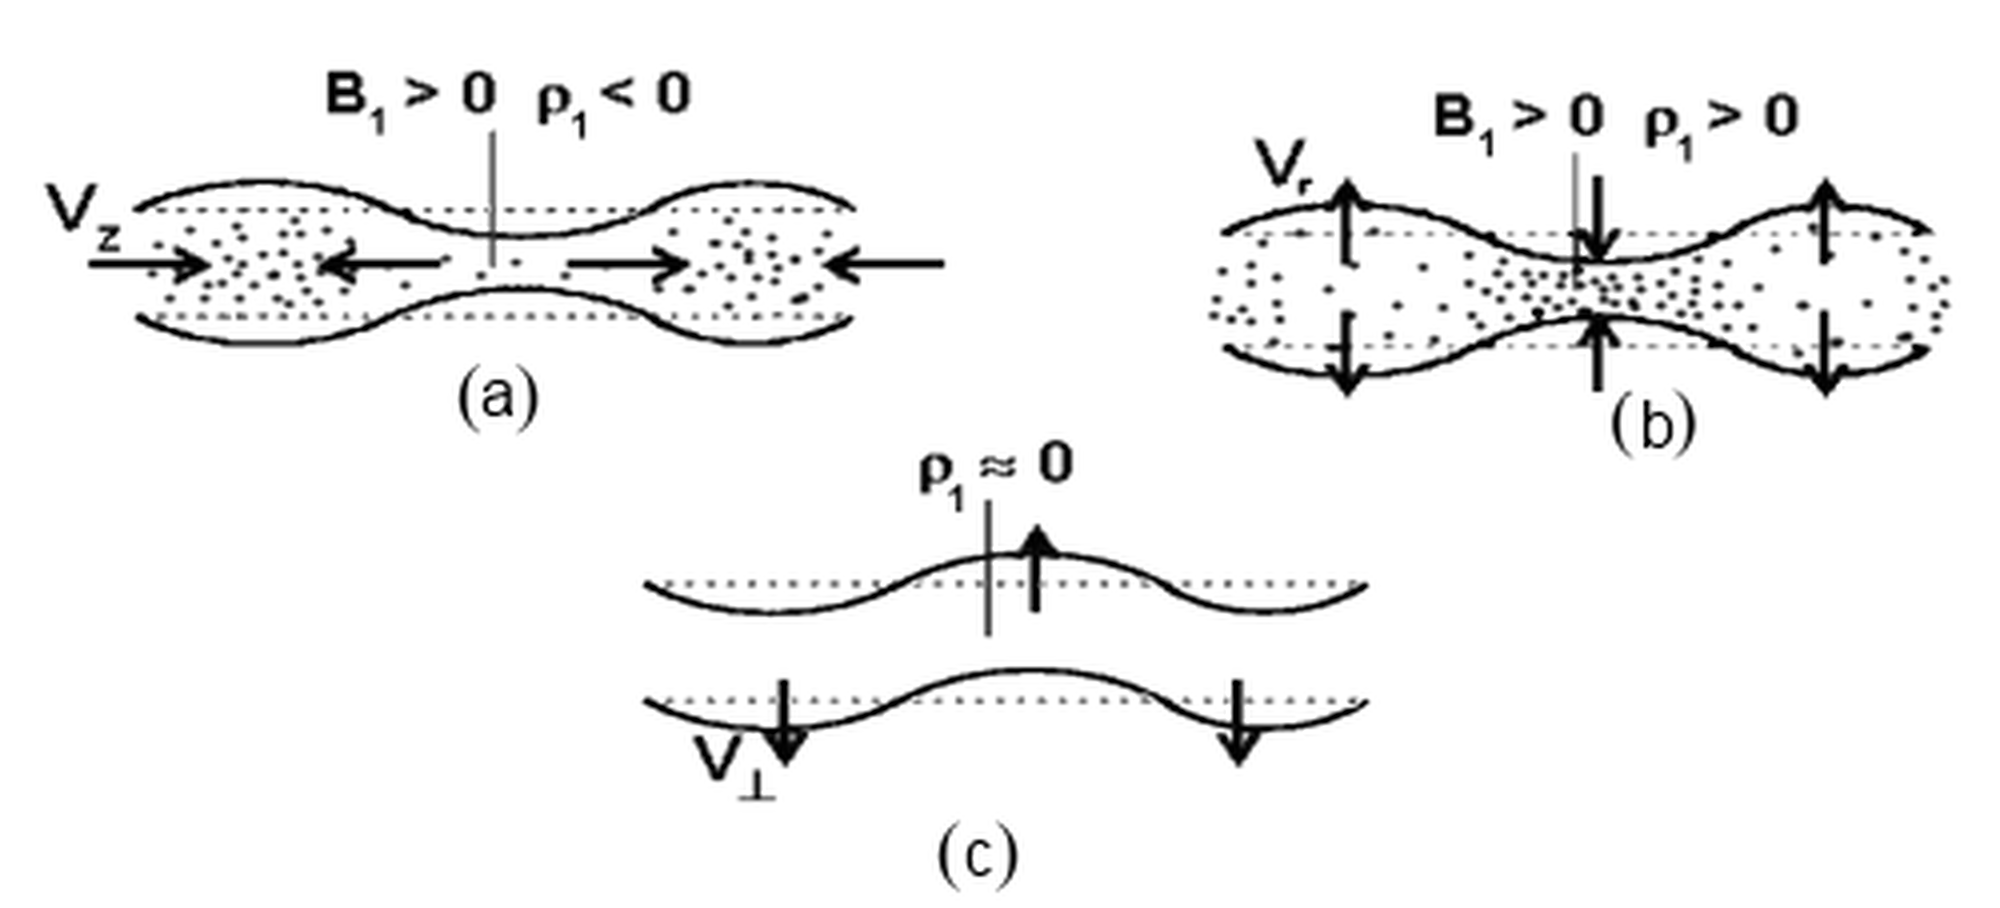
\includegraphics[width=\textwidth]{tube}
        \caption{
                 The physical effects that each type of wave has on the flux tube.
                 (a) The slow magneto-acoustic waves (slow sausage mode) which cause anti-phase behaviour between the intensity and the magnetic field.
                 (b) The fast magneto-acoustic waves (fast sausage mode) which cause in-phase behaviour between the intensity and the magnetic field.
                 (c) The fast magneto-acoustic waves (fast kink mode) which cause no magnetic field perturbations but cause $\pi/2$ phase behaviour between the intensity and velocity perturbation.
                 Image is a modified version of Figure 1 from \cite{CLOO}.
                }
        \label{fig:tube}
    \end{figure}
      
    \begin{table}
        \centering
        \begin{tabular}{l|c|c|c|c}
            &$\phi_{\mathrm{B}}-\phi_{\mathrm{v}}$&$\phi_{\mathrm{v}}-\phi_{\mathrm{I}}$&$\phi_{\mathrm{I}}-\phi_{\mathrm{B}}$&$\phi_{\mathrm{S}}-\phi_{\mathrm{I}}$ \\ \hline\hline
        Slow sausage propagating        & $\pi$ & 0 & $\pi$ & 0 \\
        Slow sausage standing           & $\pm\pi/2$ & $\pm\pi/2$ & $\pi$ & 0 \\
        Fast sausage propagating$^6$    & [0,$\pi$] & [$-\pi/2$,0] & [$-\pi/2$,0] & $\pi$ \\
        Fast sausage standing$^6$       & $\pm\pi/2$ & $\pm\pi/2$ & [0,$\pi$] & $\pi$  \\
        Fast kink propagating       	& $\pm\pi/2^3$ & $N/A^4$ & $N/A^4$ & $N/A^4$ \\
        Fast kink standing          	& [$\pi/2^1,\pi^2$] & $N/A^4$ & $N/A^4$ & $N/A^4$ \\ \hline
        \end{tabular}
        \caption{
            Shows the phase differences between three observables: the intensity, Doppler velocity and the magnetic field for each type of MHD wave and whether the wave is standing (S) or propagating (P).
            1 - Wave propagating anti-parallel to the magnetic field.
            2 - Wave propagating parallel to the magnetic field. 
            3 - Depending on the distance to the reflection boundary.
            4 - Kink modes are incompressible and thus have zero intensity fluctuations.
            5 - Fast sausage mode has zero LOS velocity fluctuations.
            6 - Surface mode only.
            Collated from these authors, \cite{CLOO,PMHDW,Moreels2013,Moreels2013b,2015A&A...579A..73M}}
        \label{tab:phase}
    \end{table}